\documentclass[a4paper]{article}
\usepackage{exercise}
%um nur aufgaben zu zeigen
%\usepackage[noanswer]{exercise} 
\usepackage{../images/preamble}
\usepackage{rotating}
\usetikzlibrary{decorations.pathmorphing}
\usetikzlibrary{decorations.markings}
\usetikzlibrary{arrows}
\usetikzlibrary{shapes.geometric}
\newcommand{\midarrow}{\tikz \draw[-triangle 90] (0,0) -- +(.02,0);}
\usepackage{xcolor}
%\usepackage{draftwatermark}
%\SetWatermarkText{\textsc{Draft 2}}
%\SetWatermarkScale{3}
%\SetWatermarkColor{red!30}


\usepackage[printwatermark]{xwatermark}
%\newsavebox\mybox
%\savebox\mybox{\tikz[color=red,opacity=0.3]\node{\textsc{Entwurf}};}
%\newwatermark*[
%allpages,
%angle=45,
%scale=10,
%xpos=-4cm,
%ypos=4cm
%]{\usebox\mybox}
\pagestyle{fancy}
\fancyhead[L]{\includegraphics[width=2cm]{../images/logo_scaled.pdf}}
\fancyhead[R]{\textsc{Aufgabenserie 6}}


\begin{document}
	\vspace*{-1cm}
	\parbox{4cm}{\vspace{-0.2cm}\includegraphics[width=5cm]{../images/logo_scaled.pdf}}
	\parbox{10.6cm}{\setstretch{2.0} \centering{ \huge \textsf{Aufgabenserie 6 
			}}\\
			Abgabe: 8. April 2018 \\ \vspace*{-.5cm} }
		\vspace{0.5cm}

\thispagestyle{empty}
\begin{framed}
	\noindent
	\scriptsize
	Die Aufgaben sollten bis zum \textbf{8. April} bearbeitet werden. Die Lösungen schickt ihr an \href{mailto:physikrolf@gmail.com}{physikrolf@gmail.com}.\\ Die aktuellen Aufgaben sowie alle alten Aufgabenserien mit Lösungen findet ihr auch auf \url{pankratius.github.io/rolf}.
\end{framed}

\noindent

\begin{minipage}[b]{0.8\textwidth}
\begin{Exercise}[title = Zwei Pucks, origin = {Morin - Classical Mechanics}, difficulty = 3, label = pucks]
Ein masseloser Faden der Länge $2\ell$ verbindet zwei Hockeypucks, die auf einer reibungsfreien Eisfläche liegen.\\
Jemand zieht mit einer konstanten Kraft $\vec{F}$ an der Mitte des Seils, wobei die Kraft senkrecht angreift.
Nach einer gewissen Zeit stoßen die beiden Pucks komplett inelastisch zusammen. Wie viel Energie geht bei dem Stoß verloren?
\end{Exercise}
\end{minipage}
\hfill
\begin{minipage}[b]{.2\textwidth}
\centering
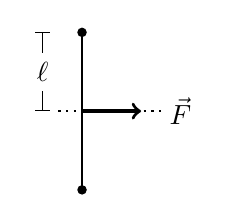
\begin{tikzpicture}
\filldraw (0,1) circle (1.5pt);
\draw (0,1) -- (0,-1);
\filldraw (0,-1) circle (1.5pt);
\draw[->,very thick] (0,0) --  (0.75,0);
\node at (1.25,0) {$\vec{F}$};
\draw[|-|] (-.5,1) to node[midway, fill = white] {$\ell$} (-.5,0);
\draw[dotted, thick] (-.3,0) -- (1,0);
\end{tikzpicture}
\end{minipage}
\begin{Answer}[ref = pucks]
	Diese Aufgabe kann, mal wieder, mit und ohne Analysis lösen.\\
	Mit Analysis geht das so: Wir bezeichnen den Winkel zwischen dem Puck und der Bewegungsrichtung des Seils mit $\theta$.\\
\end{Answer}
\begin{Exercise}[title = Lichtband, label = band, difficulty = 3, origin = {1. Runde im Auswahlwettbewerb zur IPhO 2006}]
Eine Lichtquelle in Form eines dünnen Bandes der Länge $\ell = 10~\mathrm{cm}$ liegt auf der optischen Achse einer dünnen Sammellinse der Brennweite $f = 5~\mathrm{cm}$ und dem Durchmesser $d = 1~\mathrm{cm}$. Der minimale Abstand der Lichtquelle zur Sammellinse beträgt $10~\mathrm{cm}$. Wie groß ist der minimale Durchmesser des entstehenden Lichtflecks, den die Lichtquelle auf einem senkrecht zur optischen Achse stehenden, verschiebbaren Schirm erzeugt?
\end{Exercise}
\begin{Exercise}[title = Tunnel, origin = {EstPhO 2009}, difficulty = 3, label = train]
	Ein Zug fährt mit einer Geschwindigkeit $v$ und einer Leistung $P$ durch einen langen zylindrischen Tunnel, dessen halbkreisförmige Öffnung einen Durchmesser $d$ hat.\\
	Die Anfangstemperatur im Tunnel beträgt $T_0$, der Luftdruck ist $p_0$, die molare Masse von Luft ist $M$. Während der Durchfahrt bleibt der Druck im Tunnel näherungsweise konstant. Dann ist die molare Wärmekapazität von Luft durch $C_p$ gegeben.\\
	Welche Temperatur hat die Luft im Tunnel nach der Zugdurchfahrt?\\
	\textit{Hinweis: Wie schon auf dem letzten Blatt kann die Luft auch in dieser Aufgabe als \textit{ideales Gas} angenommen werden. Das heißt insbesondere auch, dass die Gleichung $pV = NRT$ für die Luft erfüllt ist. \\
	Dabei ist $p$ der Gasdruck, $V$ das Volumen, $N$ die Stoffmenge und $T$ die Temperatur der Luft. $R$ ist die sog. idelle Gaskonstante. Für zweiatomige Gase wie Luft gilt in guter Näherung $C_P = \nicefrac{7}{2}\cdot R$.}
\end{Exercise}


\end{document}